\section{Software correlator}\label{sec:softwarecorrelation}
If the data in an {\it e}-VLBI experiment can be streamed over the
internet to JIVE, it can also be sent to another correlator. Within
\scarie, we are investigating the possibilities of a next generation
software correlator using a computing Grid. A similar attempt is
presented in \cite{deller-2007}. The advantages of a software
correlator over a new dedicated hardware correlator lie in its
flexibility and accuracy. The main advantage of a dedicated hardware
correlator is the greater performance. The flexibility of its
architecture allows the software correlator to change with the
individual needs of researchers. In fact, the first version of the
software correlator was developed to track the Huygens spacecraft
during its descent through the atmosphere of Saturn's moon Titan. Due
to the nature of this experiment, special requirements are put on the
correlator, which the current hardware correlator is not able to
provide.  Moreover, we expect that the costs of developing a software
correlator are much lower than the costs for a hardware correlator.

\begin{comment}
  The advance of general purpose computing is making software
  correlation a cost-effective solution for a range of applications.
\end{comment}

Currently, the software correlator is used in the production
environment for doing ftp-fringe tests. Since the EVN is an ad-hoc
array, the telescopes are reconnected before every VLBI-session. In
order to test the network, the telescopes observe a well known source
and transmit the data to JIVE where it is processed immediately. The
EVN ftp fringe tests provide quick feedback to the stations on their
performance.

Computationally the correlation is relatively inexpensive, in the
sense that it requires only few operations per transferred bytes.
However, due to the high data rates, the absolute number of clock
cycles required by the application is still extremely high.  Moreover,
the problem is quadratic in the number of telescopes participating in
the experiment since it is linear in the number of channel pairs that
have to be correlated. The huge need for networking and computing
power together with it's flexibility, makes a computing Grid an ideal
platform for this application.



\begin{figure}
  \centering
  \includegraphics[width=.75\textwidth]
    {img/Network_correlator}
    \caption{Outline of the network connections between different
      components in the software correlator.}
  \label{fig:netw_corr}
\end{figure}


\subsection{Design}
In the software correlator, we split the computation in time slices.
These time slices are processed in parallel (see
Figure~\ref{fig:netw_corr}). The signal from a telescope is received
by a single so-called input node.  The input node sends slices of data
to one of the available correlator nodes. The correlator node receives
data from all telescopes for a certain time slice and performs the
correlation. The size of the output of the correlation is much smaller
than the input size and can be collected and stored by a single output
node.  There is a single manager node that assigns data to available
computing nodes.

\begin{comment}
  The software correlator is written in \verb~C++~ and uses several
  standard libraries like \verb~fftw~ \cite{FFTW05} for the fast
  Fourier transforms, \verb~mpich~ \cite{Gropp:1996:HPI} as the MPI
  implementation , \verb~GSL~ \cite{GSL} for cubic spline fitting and
  the standard template library.
\end{comment}

The manager node is the central node that controls the workflow of the
entire software correlator. It assigns time slices to available
correlator nodes and handles errors. After all time slices are
processed it terminates the software correlator.

The input node receives the data from a data stream, which can either
be a file, a TCP connection or directly from the dedicated hardware
used to record and play back the data. On request of the manager node,
it can extract the current time from the data stream or go to a
specified time. When the input node gets a request to send data for a
certain time slice to a correlator node, it seeks the right starting
sample in the input stream and sends the data to the correlator node.

The correlator node gets data for the same time slice from every input
node. First it, compensates for the fractional delay and performs the
phase rotation. These manipulations are not done on the input node
because they require floating point samples, hence the data stream
expands from 2 bits per sample to 32 bits or even 64 bits per sample,
which would require much more network bandwidth. After the fractional
delay correction and the phase rotation, the signal is ready to be
correlated.  The auto and cross correlation are then computed by
Fourier transforming the input signal and element-wise multiplying all
combination of telescope-pairs. These values are accumulated over a
certain period of time and the accumulated values are sent to the
output node.

The output node will receives the data from the correlator nodes,
sorts the data and stores it at a specified location.

%%% Local Variables:
%%% mode: latex
%%% TeX-master: "Ingrid"
%%% End:
